\chapter{Data import via ODBC}
\label{chap:odbc}

Since version 1.7.5, \app{gretl} provides a method for retrieving data
from databases which support the Open Database Connectivity (ODBC)
standard. Most users won't be interested in this, but there may be
some for whom this feature matters a lot --- typically, those who work
in an environment where huge data collections are accessible via a
Data Base Management System (DBMS).

In the following section we explain what is needed for ODBC support in
\app{gretl}. We provide some background information on how ODBC works
in section~\ref{sec:odbc-base}, and explain the details of getting
\app{gretl} to retrieve data from a database in
section~\ref{sec:odbc-syntax}.

\section{ODBC support}
\label{sec:odbc-support}

The piece of software that bridges between \app{gretl} and the ODBC
system is a dynamically loaded ``plugin''. This is included in the
\app{gretl} packages for MS Windows and Mac OS X (on OS X support was
added in \app{gretl} 1.9.0). On other unix-type platforms (notably
Linux) you will have to build \app{gretl} from source to get ODBC
support.  This is because the \app{gretl} plugin depends on
having \app{unixODBC} installed, which we cannot assume to be the
case on typical Linux systems. To enable the ODBC plugin when building 
\app{gretl}, you must pass the option \verb|--with-odbc| to
\app{gretl}'s \texttt{configure} script. In addition, if
\app{unixODBC} is installed in a non-standard location you will have
to specify its installation prefix using \verb|--with-ODBC-prefix|,
as in (for example)
\begin{code}
  ./configure --with-odbc --with-ODBC-prefix=/opt/ODBC
\end{code}

\section{ODBC base concepts}
\label{sec:odbc-base}

ODBC is short for \emph{Open DataBase Connectivity}, a group of
software methods that enable a \emph{client} to interact with a
database \emph{server}. The most common operation is when the client
fetches some data from the server. ODBC acts as an intermediate layer
between client and server, so the client ``talks'' to ODBC rather than
accessing the server directly (see Figure~\ref{fig:odbc}).

\begin{figure}[htbp]
  \centering
  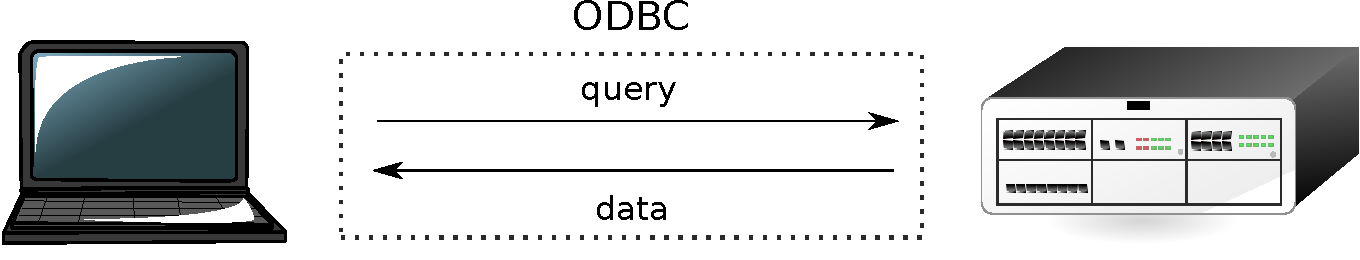
\includegraphics[width=0.8\textwidth]{figures/odbc}
  \caption{Retrieving data via ODBC}
  \label{fig:odbc}
\end{figure}

For the above mechanism to work, it is necessary that the relevant
ODBC software is installed and working on the client machine (contact
your DB administrator for details). At this point, the database (or
databases) that the server provides will be accessible to the client
as a \emph{data source} with a specific identifier (a Data Source Name
or DSN); in most cases, a username and a password are required to
connect to the data source.

Once the connection is established, the user sends a \emph{query} to
ODBC, which contacts the database manager, collects the results and
sends them back to the user. The query is almost invariably formulated
in a special language used for the purpose, namely SQL.\footnote{See
  \url{http://en.wikipedia.org/wiki/SQL}.} We will not provide here an
SQL tutorial: there are many such tutorials on the Net; besides, each
database manager tends to support its own SQL dialect so the precise
form of an SQL query may vary slightly if the DBMS on the other end is
Oracle, MySQL, PostgreSQL or something else.

Suffice it to say that the main statement for retrieving data is the
\texttt{SELECT} statement.  Within a DBMS, data are organized in
\emph{tables}, which are roughly equivalent to spreadsheets. The
\texttt{SELECT} statement returns a subset of a table, which is itself
a table. For example, imagine that the database holds a table called
``NatAccounts'', containing the data shown in
Table~\ref{tab:odbc-nataccounts}.

\begin{table}[htbp]
  \centering
  \begin{tabular}{rrrrr}
    \hline
    year	& qtr	& gdp	 & consump	& tradebal \\ 
    \hline
    1970	& 1	& 584763 & 344746.9	& $-$5891.01 \\ 
    1970	& 2	& 597746 & 350176.9	& $-$7068.71 \\ 
    1970	& 3	& 604270 & 355249.7	& $-$8379.27 \\ 
    1970	& 4	& 609706 & 361794.7	& $-$7917.61 \\ 
    1971	& 1	& 609597 & 362490	& $-$6274.3  \\ 
    1971	& 2	& 617002 & 368313.6	& $-$6658.76 \\ 
    1971	& 3	& 625536 & 372605	& $-$4795.89 \\ 
    1971	& 4	& 630047 & 377033.9	& $-$6498.13  
  \end{tabular}
  \caption{The ``NatAccounts'' table}
  \label{tab:odbc-nataccounts}
\end{table}

The SQL statement
\begin{code}
  SELECT qtr, tradebal, gdp FROM NatAccounts WHERE year=1970;
\end{code}
produces the subset of the original data shown in Table~\ref{tab:odbc-result}.

\begin{table}[htbp]
  \centering
  \begin{tabular}{rrrrr}
    \hline
    qtr	& tradebal & gdp    \\ 
    \hline
    1	& $-$5891.01 & 584763 \\ 
    2	& $-$7068.71 & 597746 \\ 
    3	& $-$8379.27 & 604270 \\ 
    4	& $-$7917.61 & 609706  
  \end{tabular}
  \caption{Result of a \texttt{SELECT} statement}
  \label{tab:odbc-result}
\end{table}

\app{Gretl} provides a mechanism for forwarding your query to the DBMS
via ODBC and including the results in your currently open dataset.

\section{Syntax}
\label{sec:odbc-syntax}

At present \app{gretl} does not offer a graphical interface for ODBC
import; this must be done via the command line interface. The two
commands used for fetching data via an ODBC connection are
\texttt{open} and \texttt{data}.

The \texttt{open} command is used for connecting to a DBMS: its syntax
is
\begin{flushleft}
\texttt{%
  open dsn=\emph{database} [user=\emph{username}]
  [password=\emph{password}] --odbc
}
\end{flushleft}
The \texttt{user} and \texttt{password} items are optional; the effect
of this command is to initiate an ODBC connection. It is assumed that
the machine \app{gretl} runs on has a working ODBC client installed.

In order to actually retrieve the data, the \texttt{data} command is
used. Its syntax is:
\begin{flushleft}
\texttt{%
  data \emph{series} [obs-format=\emph{format-string}] query=\emph{query-string} --odbc
}
\end{flushleft}
where:
\begin{description}
\item[\emph{series}] is a list of names of gretl series to contain the
  incoming data, separated by spaces.  Note that these series need not
  exist pior to the ODBC import.
\item[\emph{format-string}] is an optional parameter, used to handle
  cases when a ``rectangular'' organisation of the database cannot be
  assumed (more on this later);
\item[\emph{query-string}] is a string containing the SQL statement
  used to extract the data.\footnote{Prior to \app{gretl} 1.8.8, the
    tag ``\texttt{query=}'' was not required (or accepted) before the query
    string, and only one series could be imported at a time.  This
    variant is still accepted for the sake of backward compatibility.}
\end{description}
%
There should be no spaces around the equals signs in the
\texttt{obs-format} and \texttt{query} fields in the \texttt{data}
command.

The \texttt{\emph{query-string}} can, in principle, contain any valid
SQL statement which results in a table. This string may be specified
directly within the command, as in
\begin{code}
  data x query="SELECT foo FROM bar" --odbc
\end{code}
which will store into the gretl variable \texttt{x} the content of the
column \texttt{foo} from the table \texttt{bar}. However, since in a
real-life situation the string containing the SQL statement may be
rather long, it may be best to store it in a string variable.  For
example:
\begin{code}
  string SqlQry = "SELECT foo1, foo2 FROM bar"
  data x y query=SqlQry --odbc
\end{code}

\subsection{The observation format specifier}

If the optional parameter \texttt{obs-format} is absent, as in the
above example, the SQL query should return $k$ columns of data, where
$k$ is the number of series names listed in the \texttt{data} command.
It may be necessary to include a \texttt{smpl} command before the
\texttt{data} command to set up the right ``window'' for the incoming
data.  In addition, if one cannot assume that the data will be
delivered in the correct order (typically, chronological order), the
SQL query should contain an appropriate \texttt{ORDER BY} clause.

The optional format string is used for those cases when there is no
certainty that the data from the query will arrive in the same order
as the \app{gretl} dataset. This may happen when missing values are
interspersed within a column, or with data that do not have a natural
ordering, e.g.\ cross-sectional data. In this case, the SQL statement
should return a table with $m+k$ columns, where the first $m$
columns are used to identify the observation or row in the \app{gretl}
dataset into which the actual data values in the final $k$ columns
should be placed.  The \texttt{obs-format} string is used to translate
the first $m$ fields into a string which matches the string
\app{gretl} uses to identify observations in the currently open
dataset. Up to three columns can be used for this purpose ($m \leq
3$).

Note that the strings \app{gretl} uses to identify observations
can be seen by printing any variable ``by observation'', as in
%
\begin{code}
print index --byobs
\end{code}
%
(The series named \texttt{index} is automatically added to a dataset
created via the \texttt{nulldata} command.)

The format specifiers available for use with \texttt{obs-format} are
as follows:

\begin{center}
\begin{tabular}{ll}
\texttt{\%d} & print an integer value \\
\texttt{\%s} & print an string value \\
\texttt{\%g} & print a floating-point value \\
\end{tabular}
\end{center}

In addition the format can include literal characters to be passed
through, such as slashes or colons, to make the resulting string
compatible with \app{gretl}'s observation identifiers.

For example, consider the following fictitious case: we have a
5-days-per-week dataset, to which we want to add the stock index for
the Verdurian market;\footnote{See
  \url{http://www.almeopedia.com/index.php/Verduria}.} it so
happens that in Verduria Saturdays are working days but Wednesdays are
not. We want a column which does \emph{not} contain data on
Saturdays, because we wouldn't know where to put them, but at the same
time we want to place missing values on all the Wednesdays.

In this case, the following syntax could be used
%
\begin{code}
  string QRY="SELECT year,month,day,VerdSE FROM AlmeaIndexes"
  data y obs-format="%d/%d/%d" query=QRY --odbc
\end{code}
%
The column \texttt{VerdSE} holds the data to be fetched, which will go
into the \app{gretl} series \texttt{y}. The first three columns are
used to construct a string which identifies the day. Daily dates take
the form \texttt{YYYY/MM/DD} in \app{gretl}.  If a row from the DBMS
produces the observation string \texttt{2008/04/01} this will match OK
(it's a Tuesday), but \texttt{2008/04/05} will not match since it is a
Saturday; the corresponding row will therefore be discarded.  On the
other hand, since no string \texttt{2008/04/23} will be found in the
data coming from the DBMS (it's a Wednesday), that entry is left blank
in our series \texttt{y}.

\section{Examples}
\label{sec:examples}

\begin{table}[htbp]
  \centering
  \begin{tabular}{p{0.4\textwidth}p{0.4\textwidth}}
  Table \texttt{Consump} &
  Table \texttt{DATA} \\
    
\begin{tabular}{ll}
\hline
 Field   & Type           \\ 
\hline 
 time    & decimal(7,2)   \\ 
 income  & decimal(16,6) \\ 
 consump & decimal(16,6) \\
\hline
\end{tabular} &

\begin{tabular}{ll}
\hline
 Field   & Type           \\ 
\hline 
 year    & decimal(4,0)  \\ 
 qtr     & decimal(1,0)  \\ 
 varname & varchar(16)   \\ 
 xval    & decimal(20,10)\\ 
\hline
\end{tabular}

  \end{tabular}

  \caption{Example AWM database -- structure}
  \label{tab:odbc-AWMexample1}
\end{table}

\begin{table}[htbp]
  \centering
  \begin{tabular}{p{0.475\textwidth}p{0.475\textwidth}}
  Table \texttt{Consump} &
  Table \texttt{DATA} \\
    
\begin{tabular}{lll}
  1970.00	& 424278.975500	& 344746.944000 \\ 
  1970.25	& 433218.709400	& 350176.890400 \\ 
  1970.50	& 440954.219100	& 355249.672300 \\ 
  1970.75	& 446278.664700	& 361794.719900 \\ 
  1971.00	& 447752.681800	& 362489.970500 \\ 
  1971.25	& 453553.860100	& 368313.558500 \\ 
  1971.50	& 460115.133100	& 372605.015300 \\ 
\ldots \\ 
\end{tabular} &

\begin{tabular}{lllr}
1970	& 1	& CAN	& $-$517.9085000000\\ 
1970	& 2	& CAN	& 662.5996000000 \\ 
1970	& 3	& CAN	& 1130.4155000000\\ 
1970	& 4	& CAN	& 467.2508000000 \\ 
1970	& 1	& COMPR	& 18.4000000000  \\ 
1970	& 2	& COMPR	& 18.6341000000  \\ 
1970	& 3	& COMPR	& 18.3000000000  \\ 
1970	& 4	& COMPR	& 18.2663000000  \\ 
1970	& 1	& D1	& 1.0000000000   \\ 
1970	& 2	& D1	& 0.0000000000   \\ 
\ldots \\ 
\end{tabular}
\end{tabular}
  \caption{Example AWM database --- data}
  \label{tab:odbc-AWMexample2}
\end{table}

In the following examples, we will assume that access is available to
a database known to ODBC with the data source name ``AWM'', with
username ``Otto'' and password ``Bingo''. The database ``AWM''
contains quarterly data in two tables (see \ref{tab:odbc-AWMexample1}
and \ref{tab:odbc-AWMexample2}):

The table \texttt{Consump} is the classic ``rectangular'' dataset;
that is, its internal organization is the same as in a spreadsheet or
econometrics package: each row is a data point and each column is a
variable. The structure of the \texttt{DATA} table
is different: each record is one figure, stored in the column
\texttt{xval}, and the other fields keep track of which variable it
belongs to, for which date.

\begin{script}[htbp]
  \caption{Simple query from a rectangular table}
  \label{ex:odbc-1}
\begin{scode}
nulldata 160
setobs 4 1970:1 --time
open dsn=AWM user=Otto password=Bingo --odbc

string Qry = "SELECT consump, income FROM Consump"
data cons inc query=Qry --odbc
\end{scode}
\end{script}

Example~\ref{ex:odbc-1} shows a query for two series: first we set up
an empty quarterly dataset. Then we connect to the database using the
\texttt{open} statement. Once the connection is established we
retrieve two columns from the \texttt{Consump} table. No observation
string is required because the data already have a suitable structure;
we need only import the relevant columns.

\begin{script}[htbp]
  \caption{Simple query from a non-rectangular table}
  \label{ex:odbc-2}
\begin{scode}
string S = "select year, qtr, xval from DATA \
       where varname='WLN' ORDER BY year, qtr"
data wln obs-format="%d:%d" query=S --odbc
\end{scode}
\end{script}

In example~\ref{ex:odbc-2}, by contrast, we make use of the
observation string since we are drawing from the \texttt{DATA}
table, which is not rectangular. The SQL statement stored in the
string \texttt{S} produces a table with three columns. The
\texttt{ORDER BY} clause ensures that the rows will be in
chronological order, although this is not strictly necessary in this
case.

\begin{script}[htbp]
  \caption{Handling of missing values for a non-rectangular table}
  \label{ex:odbc-3}
\begin{scode}
string foo = "select year, qtr, xval from DATA \
       where varname='STN' AND qtr>1"
data bar obs-format="%d:%d" query=foo --odbc
print bar --byobs
\end{scode}

Example \ref{ex:odbc-3} shows what happens if the rows in
the outcome from the \texttt{SELECT} statement do not match the
observations in the currently open \app{gretl} dataset. The query
includes a condition which filters out all the data from the first
quarter. The query result (invisible to the user) would be something
like
\begin{code}
+------+------+---------------+
| year | qtr  | xval          |
+------+------+---------------+
| 1970 |    2 |  7.8705000000 | 
| 1970 |    3 |  7.5600000000 | 
| 1970 |    4 |  7.1892000000 | 
| 1971 |    2 |  5.8679000000 | 
| 1971 |    3 |  6.2442000000 | 
| 1971 |    4 |  5.9811000000 | 
| 1972 |    2 |  4.6883000000 | 
| 1972 |    3 |  4.6302000000 | 
...
\end{code}
Internally, \app{gretl} fills the variable \texttt{bar} with the
corresponding value if it finds a match; otherwise, \texttt{NA} is
used. Printing out the variable \texttt{bar} thus produces
\begin{code}
     Obs           bar

  1970:1              
  1970:2        7.8705
  1970:3        7.5600
  1970:4        7.1892
  1971:1              
  1971:2        5.8679
  1971:3        6.2442
  1971:4        5.9811
  1972:1              
  1972:2        4.6883
  1972:3        4.6302
...
\end{code}

\end{script}
